% Chapter 1

\chapter{Implementation and Data} % Main chapter title

\label{Chapter4} % For referencing the chapter elsewhere, use \ref{Chapter1} 

\lhead{Chapter 4. \emph{Implementation and Data}} % This is for the header on each page - perhaps a shortened title

\emph{In this chapter we present our work, which centers around 66 cross-validated feature engineering experiments including a baseline evaluation. The work is divided into four components: first, the procurement of HEP training data with which to perform the experiments; then, the extensions made to GROBID to facilitate our feature engineering and evaluations; next, the pipeline assembled for automating the experimentation; and finally, the different categories of feature engineering, and our reasons for choosing them.}

\section{Objectives}

As articulated in Chapter \ref{Chapter3}, GROBID manages a hierarchy of models that propagates classified information from top to bottom in a cascade. Our objectives are therefore to enhance some models within the cascade for HEP papers. It does not, on the other hand, make sense to attempt to improve all models. After all, we may assume a HEP \emph{date} is no different from dates printed in other scientific papers. Aside for feature engineering, it is hard to imagine improving performance of these models which exemplary. The same goes for names, and with little exception\footnote{It is in fact true that HEP collaborations feature in isolated references in HEP papers (see Section \ref{sec:futurework}).}, reference lists and their contents. Undoubtedly, the models with the most promising scope for improvement are the \emph{header} and \emph{segmentation} models. It is these models that address the parts of an article most distinct in HEP papers. In particular, some physical journals have recurrent styles and formats for headers sections that are distinct from others publishers. In addition, the vocabularly of a physics headers will be distinct from that papers from other branches of sceience. These should be trained for and additionally engineered for, for example through the use of dictionary-based features (see Section \ref{subsec:dicts}). Thus, the \emph{header} model may be improved for a number of reasons, including:

\begin{enumerate}
\item physics publishers present a unique format not found in CORA papers;
\item scientific collaborations as seen in HEP papers are not modelled as a header class by vanilla GROBID, and;
\item discontinuous header data (see Figure \ref{fig:articlesamples}), which may contain substantial front matter is by default neither trained nor modelled for.
\end{enumerate}

The \emph{segmentation} model may also be improved for a number of reasons:

\begin{enumerate}
\item discontinuous header data (see Figure \ref{fig:articlesamples}), which may contain substantial front matter is neither trained nor modelled for;
\item HEP collaborations entail long author lists and affiliation lists, often disjoint from the main header section, which are neither trained nor modelled for, and;
\item the dataset is small (we more than double it in Section \ref{sec:data}).
\end{enumerate}

Note that the \emph{segmentation} model is the parent model of the entire cascade, and therefore any improvement to it will benefit all other models at prediction time. Aside from being the root of the cascade, the \emph{segmentation} model is special in that it models a full line at the token level, rather than a single character string such as for the \emph{header} model. A comparison is given in Table \ref{table:headervssegmentation}. We are mindful of this distinction as we go about our feature engineering.

\begin{table}[h]
\begin{center}
\begin{tabular}{|c|c|c|}
\hline
Model & Token & Instance \\
\hline
Header & Character string & Header section \\
\hline
Segmentation & Full line & Full document \\
\hline
\end{tabular}
\caption[Comparison of token and instance entities for \emph{header} and \emph{segmentation} models. For information on \emph{fields} tagged by these models, see Section \ref{sec:grobid}.]{Evaluation results for reference segmentation}
\label{table:headervssegmentation}
\end{center}
\end{table}

Our focus is therefore on the two models, \emph{header} and \emph{segmentation}. We therefore require two separate training sets of HEP papers, one for each model. Incidentally, both models require that for each paper we produce a TEI representation and a \emph{raw} file of extracted features, as explained in Section \ref{sec:grobid}.

\section{Data Acquisition}
\label{sec:data}

At the recommendation of an INSPIRE-HEP digital library curator, we selected a set of articles deemed to be a representative sample of the database. It contains the following varieties of papers:

\begin{enumerate}
\item conference papers (no DOI);
\item conference papers (with DOI);
\item general papers;
\item miscellaneous papers (including non-English language), and;
\item collaboration papers.
\end{enumerate}

This totalled 191 papers\footnote{Originally this numbered in excess of 200, but certain papers could not be parsed by \emph{pdf2xml}.}, however according to our adjudications, we additionally removed documents deemed to be unsuitable for training, such as books. In Sections \ref{subsec:cora}, \ref{subsec:hepdatasetheader}, and \ref{subsec:hepdatasetsegmentation}, we detail the mixture of data we have assembled. The starting point for generating training data is to apply the existing, default models of GROBID on the new dataset of PDF papers. This creates the pair of TEI and \emph{raw} file for each document, as a first attempt at a ground truth, and creates a structure on which to work. The researcher must then manually correct the inevitable myriad errors to achieve a gold standard of training data. In the case of \emph{segmentation}, this involves the validation of a full document, which may contain many recurrent errors, rendering the task stupendously time-consuming, and a barrier to actual research. In the case of the header model, this is often simpler, as it involves validating a single article section. However, wherever discontinuous front matter exists, changes must be made to both the TEI and \emph{and} raw files. This firstly involves a modification to GROBID such that it extract features for all tokens rather than just those contained in the header. Then, the unseen front matter must be manually formatted and appended to the TEI file, and the corresponding features copied to the raw file. This is problematic, as there must be a one-to-one correspondence between the token in the TEI file and the features in the raw file. Hence, any copyist mistake will invoke errors at training time.

\begin{table}[h]
\begin{center}
\begin{tabular}{|c|c|c|}
\hline
Model & HEP & CORA \\
\hline
Header & 157 papers & \textbf{2506 papers} \\
\hline
Segmentation & \textbf{169 papers} & 125 papers \\
\hline
\end{tabular}
\caption[Number of training instances for each model from each dataset.]{Number of training instances for each model from each dataset.}
\label{table:headervssegmentation}
\end{center}
\end{table}

\subsection{CORA dataset}
\label{subsec:cora}
The CORA dataset (\cite{mccallum2000automating}) is a substantial dataset of some 2506 header instances. It is popular in metadata extraction studies, as creating custom training data is a stupendously time-consuming task, and has come to be a sort of standard (\cite{Peng04accurateinformation}). From One of the questions we ask in Section \ref{sec:results} is therefore, what 

\begin{enumerate}
\item the dataset is small (we more than double it in Section \ref{sec:data})
\item the dataset is small (we more than double it in Section \ref{sec:data})
\item the dataset is small (we more than double it in Section \ref{sec:data})
\item the dataset is small (we more than double it in Section \ref{sec:data})
\end{enumerate}

Despite the overall quality of the dataset, we did encounter some small mistakes, as do (\cite{Peng04accurateinformation})

\blockquote{The \emph{note} field is the one most confused with others, and upon inspection is actually labeled inconsistently in the training data.}

\subsection{HEP dataset - Header}
\label{subsec:hepdatasetheader}

For \emph{header} training data, the command for this is \texttt{createTrainingHeader}.

Modifications had to be made to GROBID to produce features for the entire document, rather than for the first two pages as per the heuristic. This was essential to obtain features for any discontinuous front matter in other parts of the document. Wherever such matter was found, it was necessary firstly to manually append to the TEI file, following the TEI XML standard, then to copy the discontinuous segments of the \emph{raw} extracted features into the master copy. Whenever a copyist mistake was made, these entailed runtime errors, and reparations had to be made.

We were therefore able to experiment with combining the two datasets of HEP papers, as well as subsampling the CORA dataset to see . After all, in spite of common wisdom that increasing the amount of training data will increase generalisation and model performance, it is not clear what effects combining different ground truths, namely CORA and HEP, will have. One may imagine that generalising over a hybrid dataset might construct a misleading model when it comes to evaluate on a pure HEP dataset, especially when the CORA set dwarfs our HEP one. Therefore one of our research questions is whether such a mixture is beneficial, and we experiment with different CORA sample sizes in Section \ref{Chapter5}.

\begin{figure}
\centering
\begin{tabular}{cc}
\subfloat[Collaboration field in header section.]{
\includegraphics[width=0.45\textwidth]{Figures/collaboration.pdf}}\label{fig:articlesamplesA}&
\subfloat[Discontinuous header data.]{
\includegraphics[width=0.45\textwidth]{Figures/eamonn.pdf}} \\
\subfloat[Collaboration author list.]{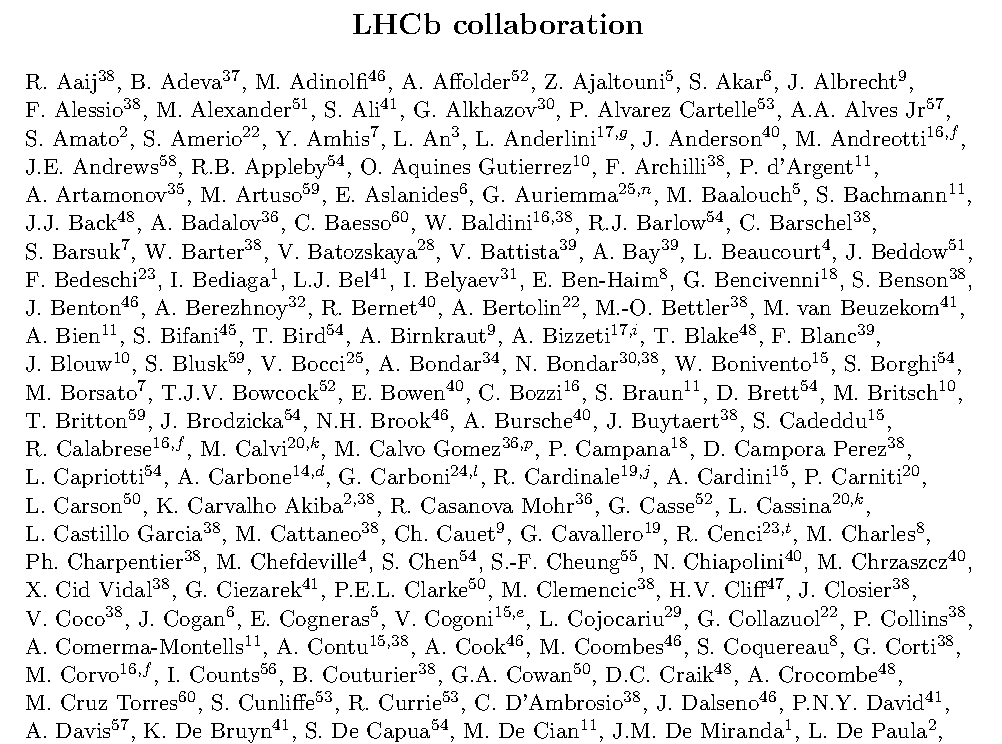
\includegraphics[width=0.45\textwidth]{Figures/authors.pdf}} & 
\subfloat[Collaboration affiliation list.]{
\includegraphics[width=0.45\textwidth]{Figures/affiliations.pdf}}\\
\end{tabular}
\caption{Figure (A) shows a collaboration field in a header section. Figure (B) shows discontinuous front matter that sits on the first page, but apart from the main header section and within the introduction section. Figures (C) and (D) give the authors list and affiliations from a large HEP collaboration; the author list begins on page . Figure (B) from (\cite{maguire2012taxonomy}), other excerpts from (\cite{aaij2015identification}).}
\label{fig:articlesamples}
\end{figure}

\subsection{HEP dataset - Segmentation}
\label{subsec:hepdatasetsegmentation}

For \emph{segmentation} training data, the command for this is \texttt{createTrainingSegmentation}. 

We were therefore able to experiment with combining the two datasets of HEP papers

\section{Extensions}

\begin{enumerate}
\item Confusion matrix
\item k worst files
\item Logging reprts
\item reconnecting header with segmentation model
\end{enumerate}

[INCLUDE SOME CODE HERE]

\section{Pipeline}

To automate the experimention process, we developed a pipeline of scripts in Python, chosen for its ubiquity in INSPIRE-HEP. The repository is open source and hosted GitHub\footnote{https://github.com/jcboyd/pykelet/src}. 

The pipeline begins with using GROBID (including all necessary extensions) to generate raw feature files for all TEI files in the ground truth dataset. These are then manually assembled into a stripped-down copy of GROBID (containing all necessary Java executables and additional data) and put into a directory, \texttt{batches/}, with other scenarios. The assemblage of training data depends on the data scenario desired. If we want to cross-vallidate over all data, we simply ensure that both \texttt{training/} and \texttt{evaluate/} directories within GROBID contain all the \emph{raw} files, and that all TEI files are in \texttt{training}. The cross validation will move a fold from the training directory to the evaluation directory, and return it when the iteration is complete. If, however, we wish to \emph{append} data for training, yet exclude it from evaluation, we ensure just to place raw files . The pipeline script will then withold for evluation only on those files present in the \texttt{evaluate/} folder. GROBID requires both TEI and raw files to be present or else they are ignored. This trick allows us to run such complex experiments without modifying GROBID or its directory structure. Each iteration of the cross-validation produces a log file of results exported from GROBID's evaluation utilities. These are then post-processed by another script that aggregates the file contents (token- and field-level performance metrics and confusion matrices) and visualises them automatically.

The scripts consist of a Python wrapper, \text{grobid.py} for GROBID, written using \texttt{pyjnius}, a library for Python enabling manipulation of Java executables using the Java Native Interface (JNI)\footnote{Certain limitations on this caused us to write a simpler \texttt{subprocess} wrapper also.}. Cross-validation (CV), \texttt{k\_fold\_cross\_validation.py} creates a \texttt{grobid} object in the following way. It uses Python mathematics library, \texttt{numpy}, to randomly shuffle data (according to a fixed seed), and then Python machine learning library \texttt{scikit-learn} to create CV folds. The folds are excluded for training and evaluated on for each iteration of CV. The output of CV is a set of log files containing results. These are processsed by a pair of scripts, [NAME HERE] and [OTHER NAME HERE] to produce visualisation of confusion matrices and performance metric comparisons.
\\
\begin{lstlisting}[language=python, caption=blabla, label={lst:grobid}]
grobid_trainer = GrobidTrainer(classpath=classpath_trainer,
                               grobid_home=grobid_home)
grobid_trainer.train(model)
grobid_trainer.evaluate(model)
\end{lstlisting}

\begin{figure}[!ht]
\center
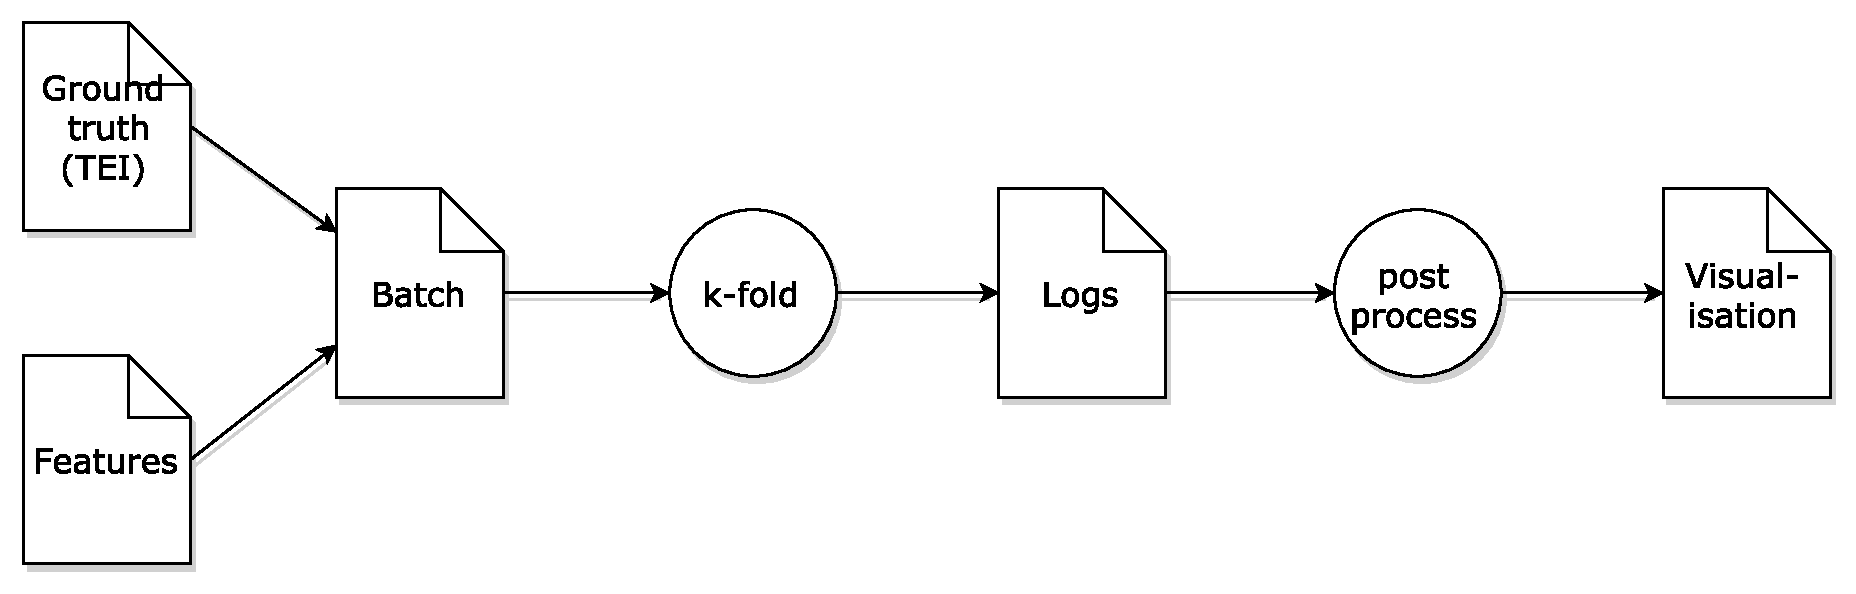
\includegraphics[width=\textwidth]{Figures/pipeline.pdf}
\caption{An illustration of the way a header section might be segmented and classified. The classes modelled are colour-coded (title in yellow, authors in green, and so on).}
\label{fig:grobid}
\end{figure}

\section{Feature Engineering}

Here we list the ideas for feature functions that we implemented and cross-validate for (see Section \ref{Chapter5}). The features were computed either by making changes to GROBID directly, or by doctoring baseline features with an external script from our pipeline (Section \ref{sec:pipeline}). In the following we use a notation consistent with that introduced in Chapter \ref{Chapter2}, that is, $x$ is a token, $\mathbf{x}$ is an instance, and $y$ and $\textbf{y}$ are the corresponding label and label vectors.

\subsection{Baseline}

To set a benchmark by which to compare our results, we ran a series of experiments including the default features for GROBID, training on different combinations of CORA and HEP data (see Section \ref{sec:experimentsetup}).

Baseline features include token identities, prefixes, suffixes, captilisation etc.

In addition, we examined the effects of ramping up the size of the CORA set appended during training.

\subsection{Block Size}

\subsection{Character Classes}

A visual scan of any scientific paper allows one to see that lines from different sections are most easily distinguished by the composition of characters. It therefore stands to reason that we can build informative features for the \emph{segmentation} model on this basis. Indeed, it may be that a line may be more effectively characterised at the \emph{character} level than the \emph{word} level. For an illustration of this effect, see Figure \ref{fig:radar}. Note that the baseline feature function set does include some basic capitalisation and punctuation indicators, but we advocate our approach for several reasons:

\begin{enumerate}
\item it is more complete in that it models more character classes;
\item it does this systematically in a feature framework that is easily modified or extended, and;
\item it performs better (see Chapter \ref{Chapter5}).
\end{enumerate}

In Table \ref{table:characterclasses}, we give a list of the character classes used to model features. The regexes were used to count the number  of characters in a token (line) belonging to each class. This was then normalised over the line length. Because such a result is numeric, we have necessarily to discretise it. We tried four different discretisation strategies: binary (according to some \emph{ad hoc} threshold), decimal (round down), decimal (round to nearest), and 20-point discretisation\footnote{In this final discretisation case we categorised results by each $5th$ percentage point, capping at $50\%$, such that we model 10 categories in total.}. For decimal case,

\begin{equation}
f_{\text{class}_i}(x_t) = \Bigg\lfloor \frac{C}{x_t}\sum_n^{|x_t|} 1_{x_t[n] \in \text{class}_i} \Bigg\rfloor,
\label{eq:classfunctions}
\end{equation}

for each character class, $\text{class}_i$, where $C$ is the discretisation factor (here $C = 10$). The other discretisation strategies may be defined similarly.

\begin{table}[h]
\begin{center}
\begin{tabular}{|c|l|l|}
\hline
Class & Regex\\
\hline
Spacing & \verb|r`[\s]'|\\
Lower case & \verb|r`[a-z]'|\\
Upper case & \verb|r`[A-Z]'|\\
Numeric & \verb|r`[\d]'|\\
Punctuation & \verb|r`[\(\).,?:;]'|\\
Special character & \verb|r`[^\sa-zA-Z\d\(\).,?:;]'|\\
\hline
\end{tabular}
\caption[Character classes used as features, along with the regular expressions used to count them.]{Character classes used as features, along with the regular expressions used to count them.}
\label{table:characterclasses}
\end{center}
\end{table}

\begin{figure}
\centering
\begin{tabular}{cc}
\subfloat[Body (formula)]{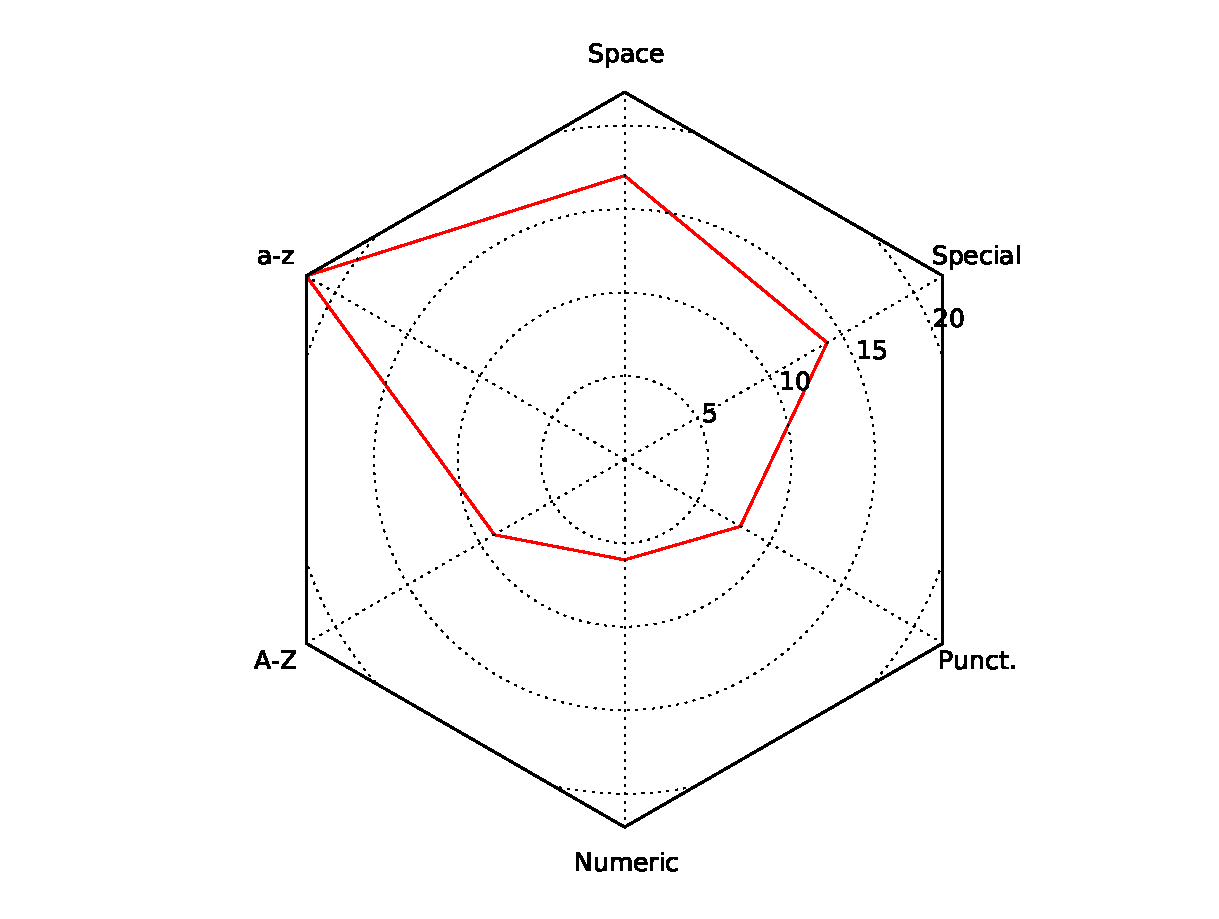
\includegraphics[width=0.5\textwidth]{Figures/body_formula.pdf}} & 
\subfloat[Body (normal)]{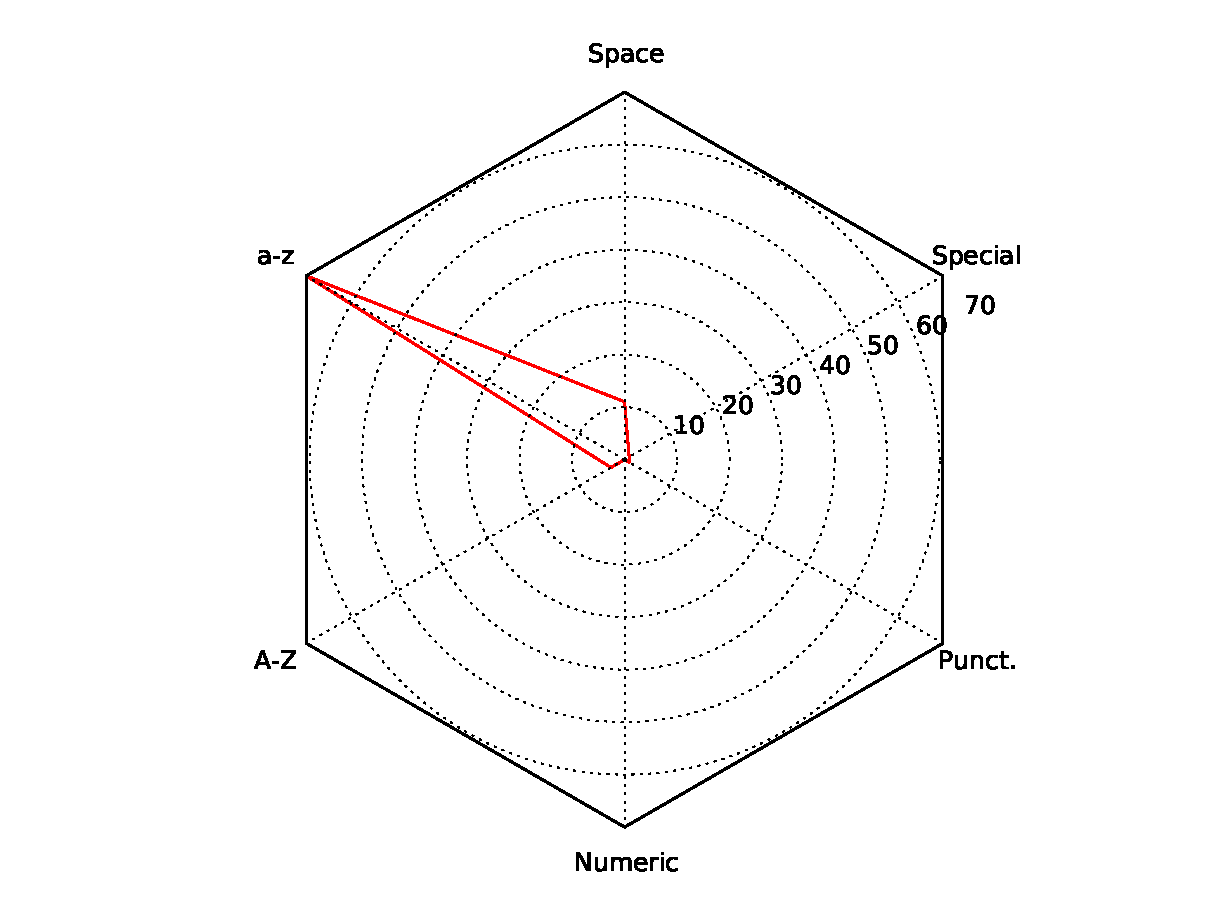
\includegraphics[width=0.5\textwidth]{Figures/body_normal.pdf}}\\
\subfloat[Headnote]{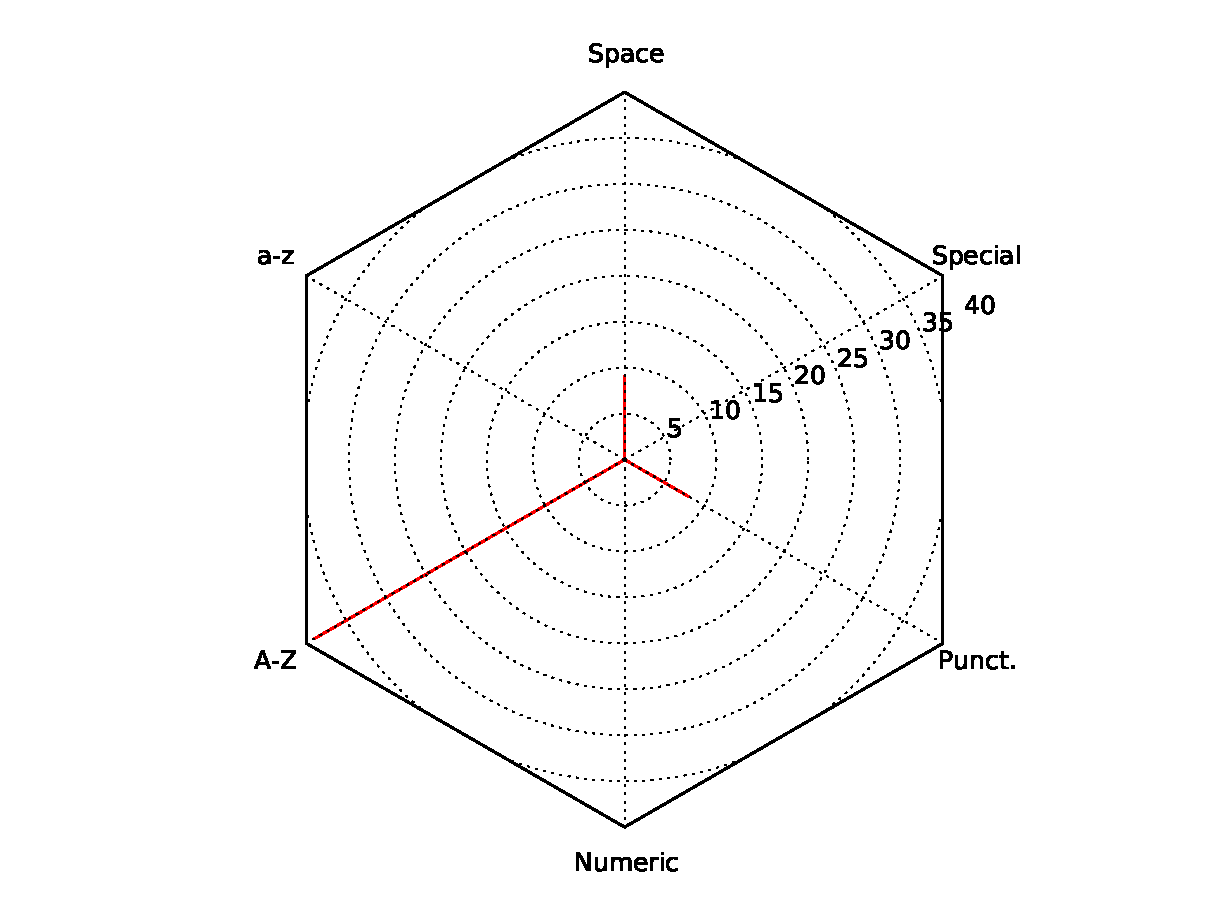
\includegraphics[width=0.5\textwidth]{Figures/headnote.pdf}}&
\subfloat[Page number]{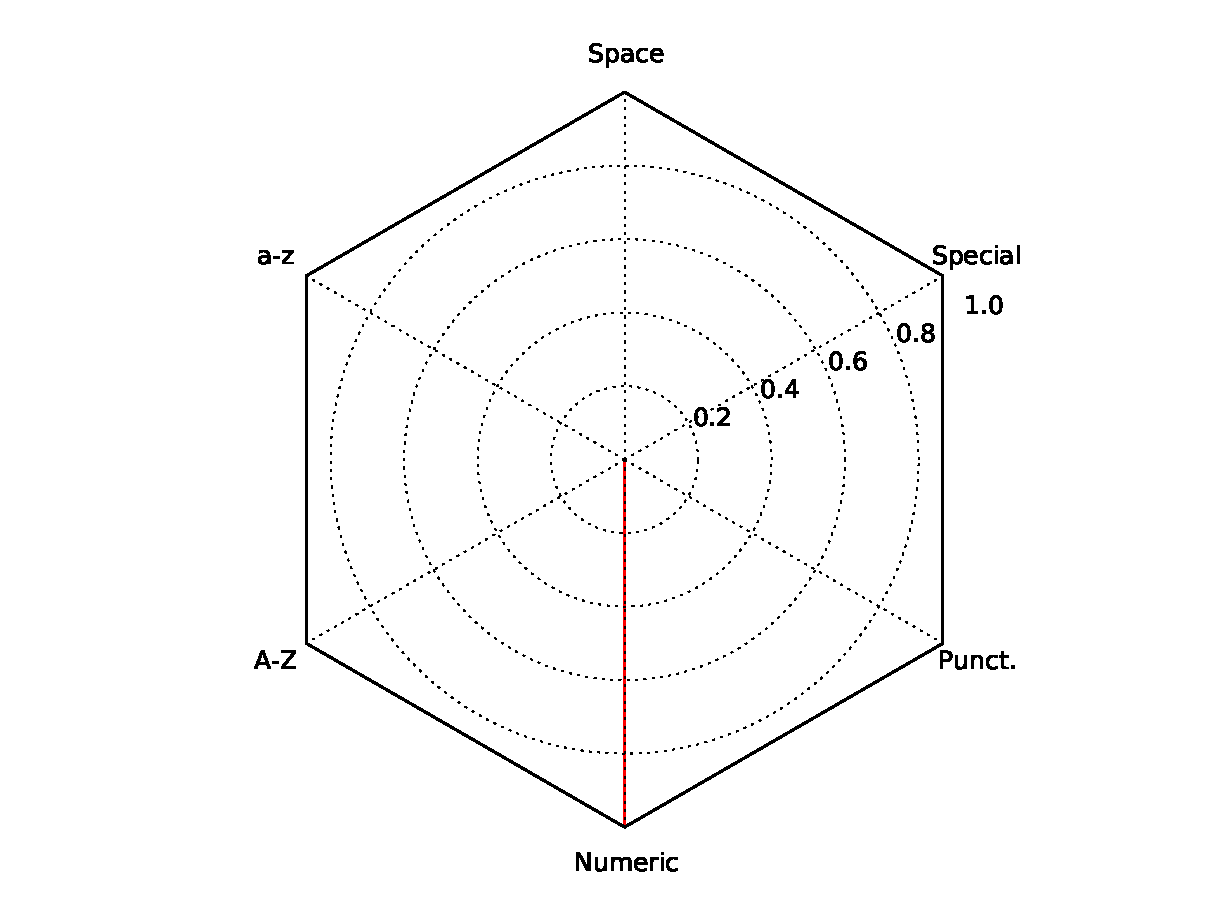
\includegraphics[width=0.5\textwidth]{Figures/page.pdf}} \\
\subfloat[Affilation list]{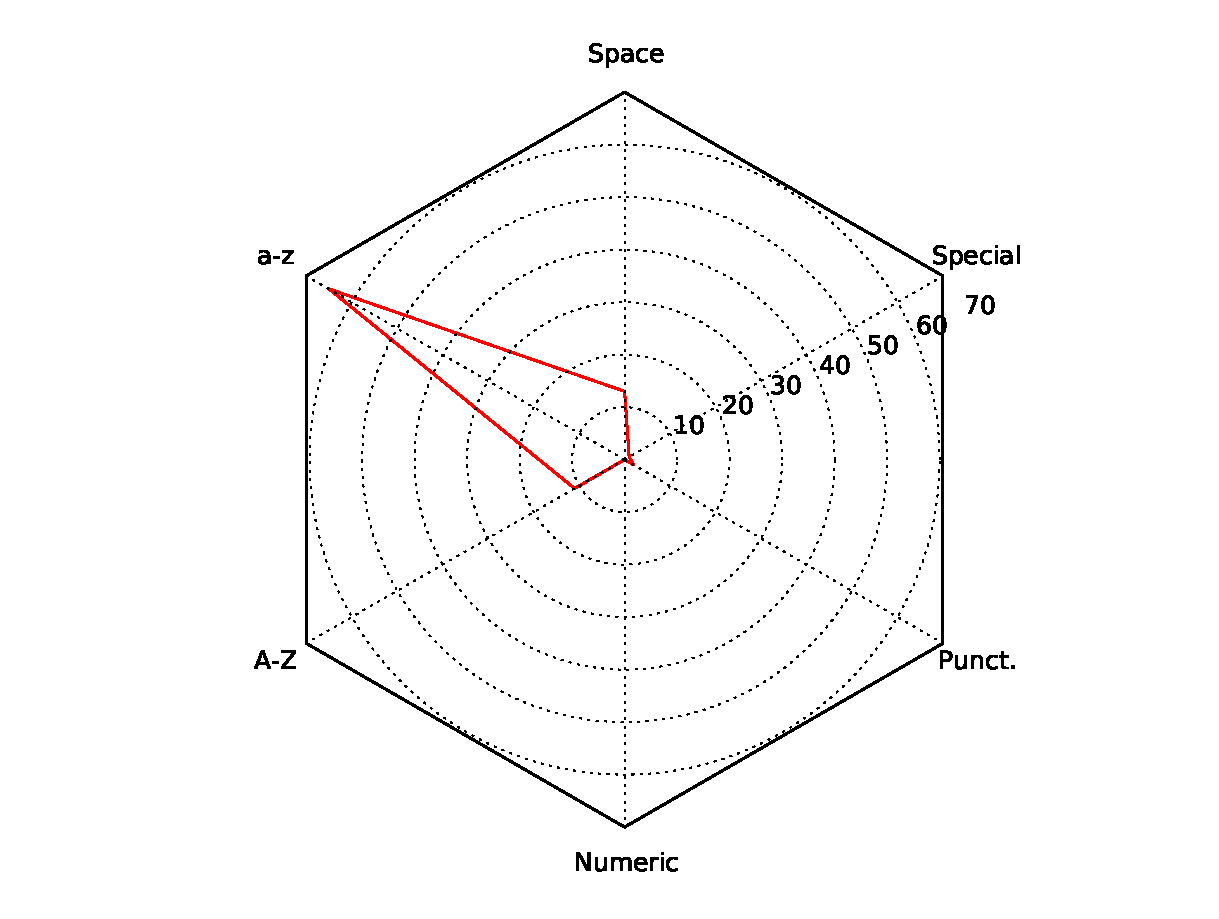
\includegraphics[width=0.5\textwidth]{Figures/affiliations_list.pdf}} & 
\subfloat[Author list]{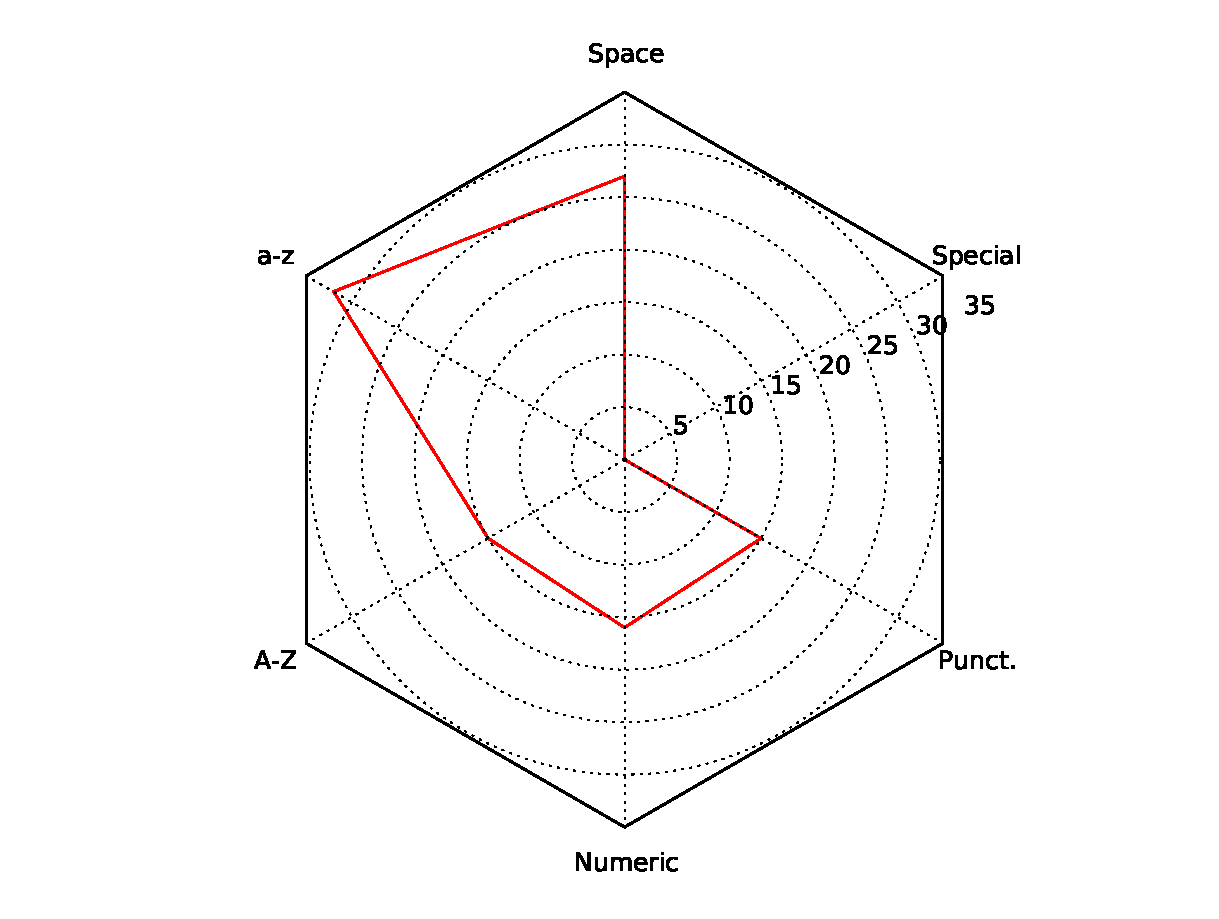
\includegraphics[width=0.5\textwidth]{Figures/author_list.pdf}} \\ 
\end{tabular}
\caption{Character class breakdown of sample lines from different sections of a CERN LHCb collaboration paper. The paper in question is the current world record holder for number of authors, and lists over 5000 authors and their affilations. The radar plots give a different impression for each of the samples.}
\label{fig:radar}
\end{figure}

\subsection{Dictionaries}
\ref{subsec:dicts}

\subsection{Dictionaries + Stops}

\subsection{Levenshtein Distance}

The Levenshtein or \emph{edit} distance can be used to quantify the edit distance between two strings, $a$ and $b$, by counting the number of changes, insertions, or deletions required for transforming $a$ into $b$. Beginning with $\text{lev}_{a, b}(|a|, |b|)$, the recursive step is defined to be,

\begin{equation}
  \text{lev}_{a, b}(i, j) = 
  \begin{cases} 
  	\text{max}(i, j) &\quad\text{if min(i, j) = 0} \\
	\text{min}
		\begin{cases}
			\text{lev}_{a, b}(i - 1, j) + 1 \\
			\text{lev}_{a, b}(i, j - 1) + 1 \\
			\text{lev}_{a, b}(i - 1, j - 1) + 1_{a_i \neq b_j} \\
		\end{cases} &\quad\text{otherwise} \\
  \end{cases}
\label{eq:levenshtein}
\end{equation}

With some exploratory data analysis we may see that the average edit distance varies between different sections, in particular at the transition points between these sections. It therefore stands to reason that the Levenshtein distance used as a feature of line tokens in the \emph{segmentation} mode. Therefore, we define a similarity measure based on the Levenshtein distance, first normalising the distance between a line and its precursor, by dividing by the length of the longer of the two, before subtracting this result from 1, to give a measure of similarity,

\begin{equation}
\text{similarity}(a, b) = 1 - \frac{\text{lev}_{a, b}(|a|, |b|)}{\text{max}(|a|, |b|)}.
\label{eq:levenshteinsimilarity}
\end{equation}

Due to the constraints on numeric features (see \ref{sec:wapiti}, we must discretised the result. Thus, for a given line, $x_t$, we define the feature function, 

\begin{equation}
  \text{f}_{lev}(x_t) =
  \begin{cases}
  	0 & \quad \text{if } 0 \leq \text{similarity}(x_t, x_{t-1}) \leq T_1 \\
	1 & \quad \text{if } T_1 \leq \text{similarity}(x_t, x_{t-1}) \leq T_2\\
	\vdots & \qquad \vdots \\
	$N-1$ & \quad \text{if } T_{N-1} \leq \text{similarity}(x_t, x_{t-1}) \leq 1 \\
  \end{cases}
\label{eq:levenshteinfunction}
\end{equation}

where $T_1, T_2, ..., T_{N-1}$ are the thresholds invoking $N$ categories. We try several thresholding strategies in our experimentation (see Section \ref{sec:experimentsetup}).

\subsection{Regularisation}

We additionally cross-validated the tuning parameter for the model, the variance for $l_2$ normalisation, $\sigma^2$, as . Unlike the true feature engineering work, this involved configuring 





\subsection{Token Extensions}

To allow this, modifications were made to GROBID to allow analysis over the full line.

